\documentclass[11pt,oneside]{article}    %use"amsart"insteadof"article"forAMSLaTeXformat
\usepackage{geometry}        %Seegeometry.pdftolearnthelayoutoptions.Therearelots.
\geometry{letterpaper}        %...ora4paperora5paperor...
%\geometry{landscape}        %Activateforforrotatedpagegeometry
%\usepackage[parfill]{parskip}        %Activatetobeginparagraphswithanemptylineratherthananindent
\usepackage{graphicx}                %Usepdf,png,jpg,orepsßwithpdflatex;useepsinDVImode
                                %TeXwillautomaticallyconverteps-->pdfinpdflatex        
\usepackage{amssymb}
\usepackage[colorlinks]{hyperref}

%----macros begin---------------------------------------------------------------
\usepackage{color}
\usepackage{amsthm}

\def\conv{\mbox{\textrm{conv}\,}}
\def\aff{\mbox{\textrm{aff}\,}}
\def\E{\mathbb{E}}
\def\R{\mathbb{R}}
\def\Z{\mathbb{Z}}
\def\tex{\TeX}
\def\latex{\LaTeX}
\def\v#1{{\bf #1}}
\def\p#1{{\bf #1}}
\def\T#1{{\bf #1}}

\def\vet#1{{\left(\begin{array}{cccccccccccccccccccc}#1\end{array}\right)}}
\def\mat#1{{\left(\begin{array}{cccccccccccccccccccc}#1\end{array}\right)}}

\def\lin{\mbox{\rm lin}\,}
\def\aff{\mbox{\rm aff}\,}
\def\pos{\mbox{\rm pos}\,}
\def\cone{\mbox{\rm cone}\,}
\def\conv{\mbox{\rm conv}\,}
\newcommand{\homog}[0]{\mbox{\rm homog}\,}
\newcommand{\relint}[0]{\mbox{\rm relint}\,}

%----macros end-----------------------------------------------------------------

\title{Boolean chains
\footnote{This document is part of the \emph{Linear Algebraic Representation with CoChains} (LAR-CC) framework~\cite{cclar-proj:2013:00}. \today}
}
\author{Alberto Paoluzzi}
%\date{}                            %Activatetodisplayagivendateornodate

\begin{document}
\maketitle
\nonstopmode

\begin{abstract}
A novel algorithm for computation of Boolean operations between cellular complexes is given in this module.
It is based on bucketing of possibly interacting geometry using a box-extension of kd-trees, normally used for  point proximity queries. 
Such kd-tree representation of containment boxes of cells, allow us to compute a number of independent buckets of data to be used for local intersection, followed by elimination of duplicated data.
Actually we reduce the intersection of boundaries in 3D to the independent intersections of the buckets of (transformed) faces with the 2D subspace $z=0$, in order to reconstruct each splitted facet of boolean arguments, suitably transformed ther together with the bucket of indent facets.
A final tagging of cells as either belonging or not to each operand follows, allowing for fast extraction of Boolean results between any pair of chains (subsets of cells).
This Boolean algorithm can be considered of a \emph{Map-Reduce} kind, and hence suitable of a distributed implementation over big datasets. The actual engineered implementation will follow the present prototype, using some distributed NoSQL database, like MongoDB or Riak. 
\end{abstract}

\tableofcontents

%===============================================================================
\section{Introduction}
%===============================================================================


%===============================================================================
\section{Preview of the algorithm}
%===============================================================================

The whole Boolean algorithm is composed by four stages in sequence, denoted in the following as \emph{Unification}, \emph{Bucketing}, \emph{Intersection}, and \emph{Reconstruction}. The algorithm described here is both multidimensional and variadic. Multidimensional means that the arguments are solid in Euclidean space of dimension $d$, with $d$ small integer.
The \emph{arity}  of a function or operation is the number of arguments or operands the function or operation accepts. 
In computer science, a function accepting a variable number of arguments is called \emph{variadic}.

\subsection{Unification}
%===============================================================================

In this first step the boundaries of the $n$ Boolean arguments are computed and merged together as a set of chains defined in the discrete set $\texttt{V}$ made by the union of their vertices, and possibly by a discrete set of points generated by intersection of cells of complementary dimension, i.e. whose dimensions add up to the dimension of the ambient space.
Actually, only the (\emph{oriented}) boundaries \texttt{V,FV$_i$} $(1\leq i\leq n)$ of the varius arguments are retained here, and used by the following steps of the algorithm.

\subsection{Bucketing}
%===============================================================================

The bounding boxes of facets \texttt{FV$_i$} are computed, and their \emph{box-kd-tree} is worked-out, so providing a group of buckets of close cells, that can be elaborated independently, and possibly in parallel, to compute the intersections of the boundary cells. 

\subsection{Intersection}
%===============================================================================

For each facet $f$ of one of Boolean arguments, the subset $F(f)$ of incident or intersecting facets of boundaries of the other arguments were computed in the previous \emph{bucketing} step. So, each $F$ is transformed by the affine map that sends $f$ into the $z=0$ subspace, and there is intersected with this subspace, generating a subset $E(f)$ of coplanar edges.
This one is projected in 2D, and the \emph{regularized} cellular 2-complex $G(f)$ induced by it is computed, and mapped back to the original space position and orientation of $f$ (providing a partition of it induced by the other boundaries).

\subsection{Reconstruction}
%===============================================================================

Like for in the reconstruction of 2D solid cells using the angular ordering of edges around the vertices, the coincident edges are identified in 3D , and used to sort the incident faces sing vhe falues of solid angles given with one reference face.
The 3D space partition induced by $\cup_f G(f)$ is finally reconstructed, possibly in parallel, by traversing the adjacent sets of facets on the boundary of each solid cell.



%===============================================================================
\section{Implementation}
%===============================================================================

\subsection{Box-kd-tree}
%===============================================================================


\paragraph{Split the boxes between the (below,above) subsets}
%-------------------------------------------------------------------------------
@D Split the boxes between the below,above subsets
@{""" Split the boxes between the below,above subsets """
def splitOnThreshold(boxes,subset,coord):
    theBoxes = [boxes[k] for k in subset]
    threshold = centroid(theBoxes,coord)
    ncoords = len(boxes[0])/2
    a = coord%ncoords
    b = a+ncoords
    below,above = [],[]
    for k in subset:
        if boxes[k][a] <= threshold: below += [k]
    for k in subset:
        if boxes[k][b] >= threshold: above += [k]
    return below,above
@}
%-------------------------------------------------------------------------------

\paragraph{Test if bucket OK or append to splitting stack}
%-------------------------------------------------------------------------------
@D Test if bucket OK or append to splitting stack
@{""" Test if bucket OK or append to splitting stack """
def splitting(bucket,below,above, finalBuckets,splittingStack):
    if (len(below)<4 and len(above)<4) or len(set(bucket).difference(below))<7 \
        or len(set(bucket).difference(above))<7: 
        finalBuckets.append(below)
        finalBuckets.append(above)
    else: 
        splittingStack.append(below)
        splittingStack.append(above)
@}
%-------------------------------------------------------------------------------


\paragraph{Remove subsets from bucket list}
%-------------------------------------------------------------------------------
@D Remove subsets from bucket list @{
""" Remove subsets from bucket list """
def removeSubsets(buckets):
    n = len(buckets)
    A = zeros((n,n))
    for i,bucket in enumerate(buckets):
        for j,bucket1 in enumerate(buckets):
            if set(bucket).issubset(set(bucket1)):
                A[i,j] = 1
    B = AA(sum)(A.tolist())
    out = [bucket for i,bucket in enumerate(buckets) if B[i]==1]
    return out

def geomPartitionate(boxes,buckets):
    geomInters = [set() for h in range(len(boxes))]
    for bucket in buckets:
        for k in bucket:
            geomInters[k] = geomInters[k].union(bucket)
    for h,inters in enumerate(geomInters):
        geomInters[h] = geomInters[h].difference([h])
    return AA(list)(geomInters)
@}
%-------------------------------------------------------------------------------
    


\paragraph{Iterate the splitting until \texttt{splittingStack} is empty}
%-------------------------------------------------------------------------------
@D Iterate the splitting until splittingStack is empty
@{""" Iterate the splitting until \texttt{splittingStack} is empty """
def boxTest(boxes,h,k):
    B1,B2,B3,B4,B5,B6,_ = boxes[k]
    b1,b2,b3,b4,b5,b6,_ = boxes[h]
    return not (b4<B1 or B4<b1 or b5<B2 or B5<b2 or b6<B3 or B6<b3)

def boxBuckets(boxes):
    bucket = range(len(boxes))
    splittingStack = [bucket]
    finalBuckets = []
    while splittingStack != []:
        bucket = splittingStack.pop()
        below,above = splitOnThreshold(boxes,bucket,1)
        below1,above1 = splitOnThreshold(boxes,above,2)
        below2,above2 = splitOnThreshold(boxes,below,2) 
               
        below11,above11 = splitOnThreshold(boxes,above1,3)
        below21,above21 = splitOnThreshold(boxes,below1,3)        
        below12,above12 = splitOnThreshold(boxes,above2,3)
        below22,above22 = splitOnThreshold(boxes,below2,3)  
              
        splitting(above1,below11,above11, finalBuckets,splittingStack)
        splitting(below1,below21,above21, finalBuckets,splittingStack)
        splitting(above2,below12,above12, finalBuckets,splittingStack)
        splitting(below2,below22,above22, finalBuckets,splittingStack)
        
        finalBuckets = list(set(AA(tuple)(finalBuckets)))
    parts = geomPartitionate(boxes,finalBuckets)
    parts = [[h for h in part if boxTest(boxes,h,k)] for k,part in enumerate(parts)]
    return AA(sorted)(parts)
@}
%-------------------------------------------------------------------------------

\paragraph{aaaaaa}
%-------------------------------------------------------------------------------
@D aaaaaa
@{""" aaaaa """

@}
%-------------------------------------------------------------------------------


\subsection{Merging the boundaries}
%===============================================================================

\subsection{Elementary splitting}
%===============================================================================

In this section we implement the splitting of $(d-1)$-faces, stored in \texttt{FV}, induced by the buckets of $(d-1)$-faces, stored in \texttt{parts}, and one-to-one associated to them. Of course, (a) both such arrays have the same number of elements, and (b) whereas \texttt{FV} contains the indices of incident vertices for each face, \texttt{parts}  contains the indices of adjacent faces for each face, with the further constraint that $i \not\in \texttt{parts}(i)$.

\paragraph{Computation of topological relations} 
The function \texttt{crossRelation} is used here to compute a topological relation starting from two characteristic matrices \texttt{XV} and \texttt{YV}, that associate the sets of topological objects $X$ and $Y$ with their vertices, respectively.
The technique using sparse binary matrices stored in \texttt{CSR} (Compressed Sparse Row) format is used.

%-------------------------------------------------------------------------------
@D Computation of topological relation
@{""" Computation of topological relation """
def crossRelation(XV,YV):
    csrXV = csrCreate(XV)
    csrYV = csrCreate(YV)
    csrXY = matrixProduct(csrXV, csrYV.T)
    XY = [None for k in range(len(XV))]
    for k,face in enumerate(XV):
        data = csrXY[k].data
        col = csrXY[k].indices
        XY[k] = [col[h] for h,val in enumerate(data) if val==2] 
        # NOTE: val depends on the relation under consideration ...
    return XY
@}
%-------------------------------------------------------------------------------
    
\paragraph{Submanifold mapping computation}
The $4\times 4$ (affine) scipy matrix \texttt{transform} of type \texttt{mat} is computed by the function \texttt{submanifoldMapping}, using as input the array \texttt{pivotFace} that contains the vertices of the so-called \emph{pivot} face, i.e.~of the face to be mapped to the coordinate subspace $z=0$ (in 3D).

%-------------------------------------------------------------------------------
@D Submanifold mapping computation
@{""" Submanifold mapping computation """
def submanifoldMapping(pivotFace):
    tx,ty,tz = pivotFace[0]
    transl = mat([[1,0,0,-tx],[0,1,0,-ty],[0,0,1,-tz],[0,0,0,1]])
    facet = [ VECTDIFF([v,pivotFace[0]]) for v in pivotFace ]
    m = faceTransformations(facet)
    mapping = mat([[m[0,0],m[0,1],m[0,2],0],[m[1,0],m[1,1],m[1,2],0],[m[2,0],
    				m[2,1],m[2,2],0],[0,0,0,1]])
    transform = mapping * transl
    return transform
@}
%-------------------------------------------------------------------------------

\paragraph{Set of line segments partitioning a facet}
The more important function of this section is the higher level \texttt{intersection} function, that accepts as input the \texttt{LAR} model \texttt{(V,FV,EV)} to be partitioned, and the pair \texttt{(k,bundledFaces)}, where \texttt{k} is the index of the pivot face (to be transformed to the $z=0$ subspace) and where \texttt{bundledFaces} is an array of indices of faces that are guarantee to share points with face $k$. Such shared points may be either boundary edges of $k$ or a segment that is internal both to face $k$ and to some face in  \texttt{bundledFaces}.

%-------------------------------------------------------------------------------
@D Set of line segments partitioning a facet
@{""" Set of line segments partitioning a facet """
def intersection(V,FV,EV):
    def intersection0(k,bundledFaces):
        FE = crossRelation(FV,EV)
        pivotFace = [V[v] for v in FV[k]]
        transform = submanifoldMapping(pivotFace)  # submanifold transformation
        transformedCells,edges,faces = [],[],[]
        for face in bundledFaces:
            edge = set(FE[k]).intersection(FE[face])  # common edge index
            if edge == set():
                print "\nk,face,FE[face] =",k,face,FE[face],"\n"
                candidateEdges = FE[face]
                for e in candidateEdges:
                    cell = [V[v]+[1.0] for v in EV[e]]  # verts of incident face
                    transformedCell = (transform * (mat(cell).T)).T.tolist()  
                    # vertices in local frame
                    transformedCells += [[point[:-1] for point in transformedCell]]
                faces = [MKPOL([cell,[range(1,len(cell)+1)],None]) 
                				for cell in transformedCells]
            else:  # boundary edges of face k
                e, = edge
                vs = [V[v]+[1.0] for v in EV[e]]
                ws = (transform * (mat(vs).T)).T.tolist()
                edges += [POLYLINE([p[:-1] for p in ws])]
        return edges,faces
    return intersection0    
@}
%-------------------------------------------------------------------------------

\paragraph{Computation of face transformations}
The faces in every $\texttt{parts}(i)$ must be affinely transformed into the subspace $x_d=0$, in order to compute the intersection of its elements with this subspace, that are submanifolds of dimension $d-2$.

%-------------------------------------------------------------------------------
@D Computation of face transformations
@{""" Computation of affine face transformations """
def COVECTOR(points):
    pointdim = len(points[0])
    plane = Planef.bestFittingPlane(pointdim,
    				[item for sublist in points for item in sublist])
    return [plane.get(I) for I in range(0,pointdim+1)]

def faceTransformations(facet):
    covector = COVECTOR(facet)
    translVector = facet[0]
    # translation 
    newFacet = [ VECTDIFF([v,translVector]) for v in facet ]
    # linear transformation: boundaryFacet -> standard (d-1)-simplex
    d = len(facet[0])
    transformMat = mat( newFacet[1:d] + [covector[1:]] ).T.I
    # transformation in the subspace x_d = 0
    out = (transformMat * (mat(newFacet).T)).T.tolist()
    print "\nin =",facet
    print "out =",out
    return transformMat
@}
%-------------------------------------------------------------------------------
    
\subsection{Boolean chains}
%===============================================================================

%===============================================================================
\section{Esporting the Library}
%===============================================================================

%-------------------------------------------------------------------------------
@O lib/py/bool2.py
@{""" Module for Boolean computations between geometric objects """
from pyplasm import *
""" import modules from larcc/lib """
import sys
sys.path.insert(0, 'lib/py/')
from inters import *
DEBUG = True

@< Coding utilities @>
@< Split the boxes between the below,above subsets @>
@< Test if bucket OK or append to splitting stack @>
@< Remove subsets from bucket list @>
@< Iterate the splitting until splittingStack is empty @>
@< Computation of face transformations @>
@< Computation of affine face transformations @>
@< Computation of topological relation @>
@< Submanifold mapping computation @>
@< Set of line segments partitioning a facet @>
@}
%-------------------------------------------------------------------------------

%===============================================================================
\section{Test examples}
%===============================================================================

\subsection{Random triangles}
%===============================================================================


\paragraph{Generation of random triangles and their boxes}
%-------------------------------------------------------------------------------
@O test/py/bool2/test01.py
@{""" Generation of random triangles and their boxes """
import sys
sys.path.insert(0, 'lib/py/')
from bool2 import *
glass = MATERIAL([1,0,0,0.1,  0,1,0,0.1,  0,0,1,0.1, 0,0,0,0.1, 100])

randomTriaArray = randomTriangles(10,0.99)
VIEW(STRUCT(AA(MKPOL)([[verts, [[1,2,3]], None] for verts in randomTriaArray])))

boxes = containmentBoxes(randomTriaArray)
hexas = AA(box2exa)(boxes)
cyan = COLOR(CYAN)(STRUCT(AA(MKPOL)([[verts, [[1,2,3]], None] for verts in randomTriaArray])))
yellow = STRUCT(AA(glass)(AA(MKPOL)([hex for hex,qualifier in hexas])))
VIEW(STRUCT([cyan,yellow]))
@}
%-------------------------------------------------------------------------------


\paragraph{Generation of random quadrilaterals and their boxes}
%-------------------------------------------------------------------------------
@O test/py/bool2/test02.py
@{""" Generation of random quadrilaterals and their boxes """
import sys
sys.path.insert(0, 'lib/py/')
from bool2 import *
glass = MATERIAL([1,0,0,0.1,  0,1,0,0.1,  0,0,1,0.1, 0,0,0,0.1, 100])

randomQuadArray = randomQuads(10,1)
VIEW(STRUCT(AA(MKPOL)([[verts, [[1,2,3,4]], None] for verts in randomQuadArray])))

boxes = containmentBoxes(randomQuadArray)
hexas = AA(box2exa)(boxes)
cyan = COLOR(CYAN)(STRUCT(AA(MKPOL)([[verts, [[1,2,3,4]], None] for verts in randomQuadArray])))
yellow = STRUCT(AA(glass)(AA(MKPOL)([hex for hex,qualifier in hexas])))
VIEW(STRUCT([cyan,yellow]))
@}
%-------------------------------------------------------------------------------

\begin{figure}[htbp] %  figure placement: here, top, bottom, or page
   \centering
   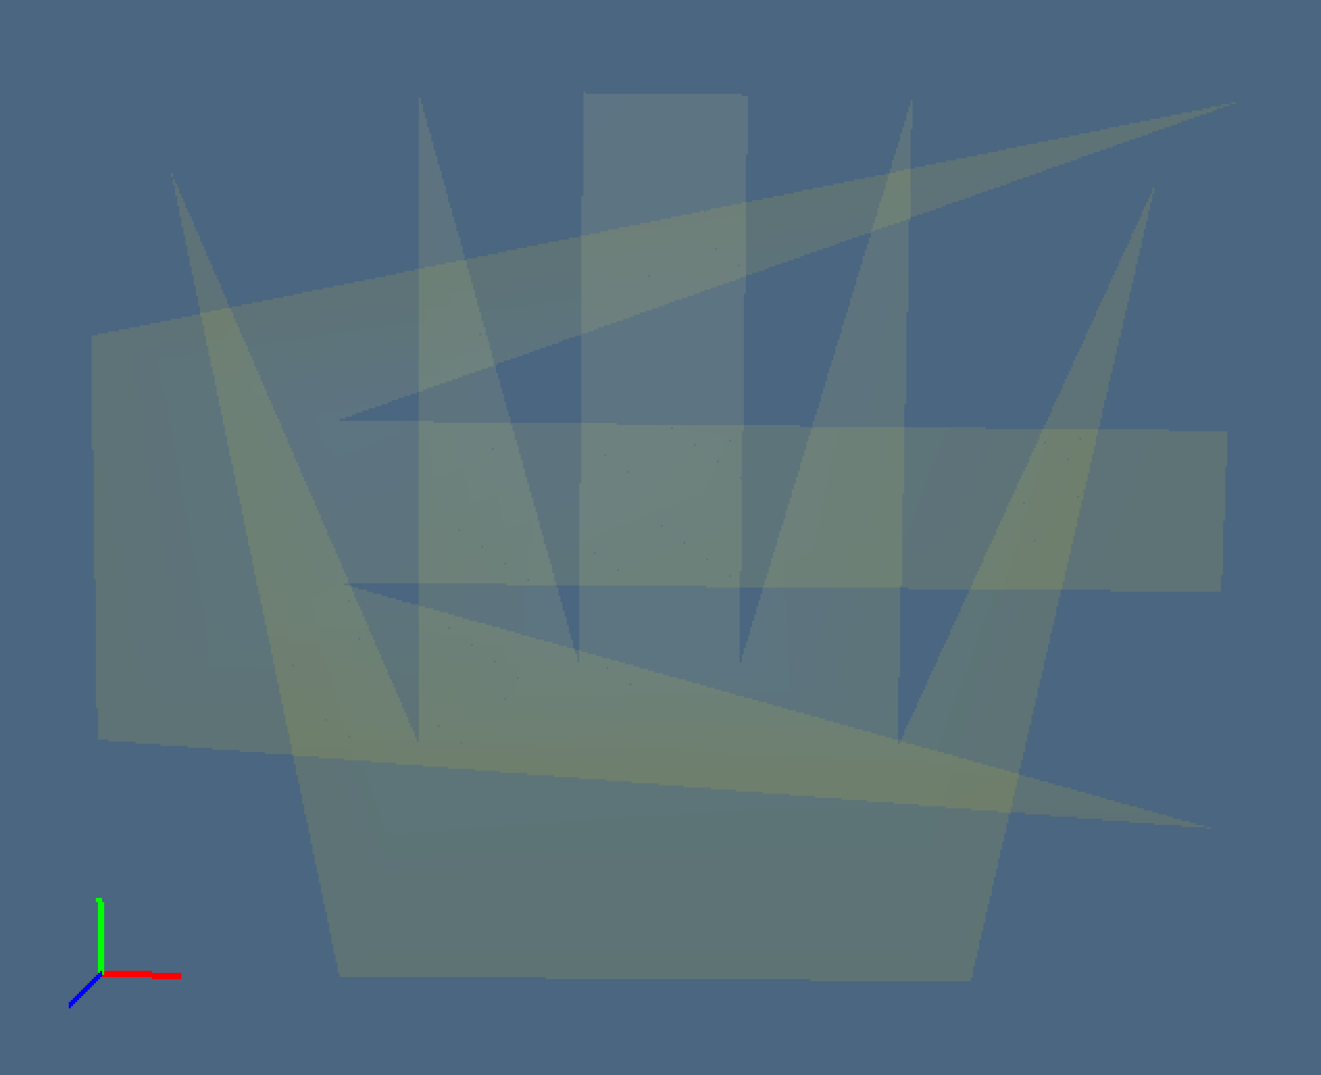
\includegraphics[height=0.2\linewidth,width=0.2425\linewidth]{images/fork1} 
   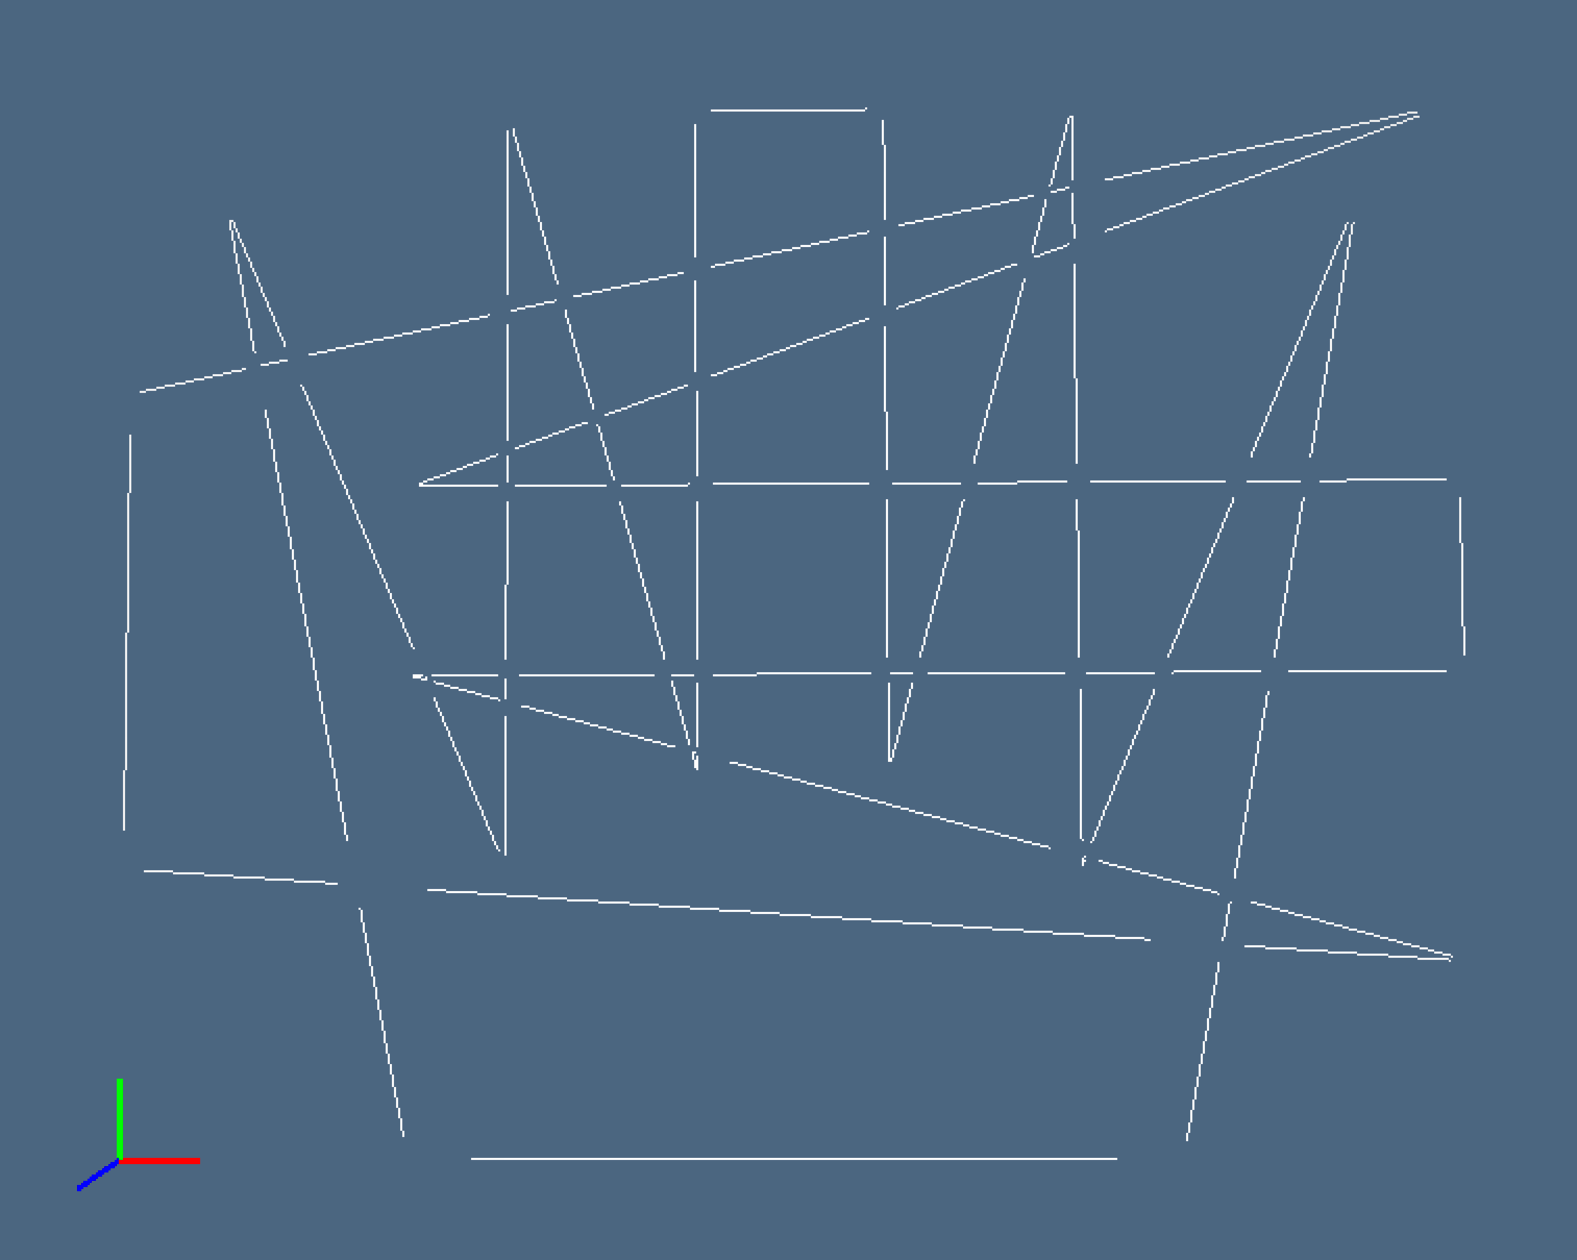
\includegraphics[height=0.2\linewidth,width=0.2425\linewidth]{images/fork2} 
   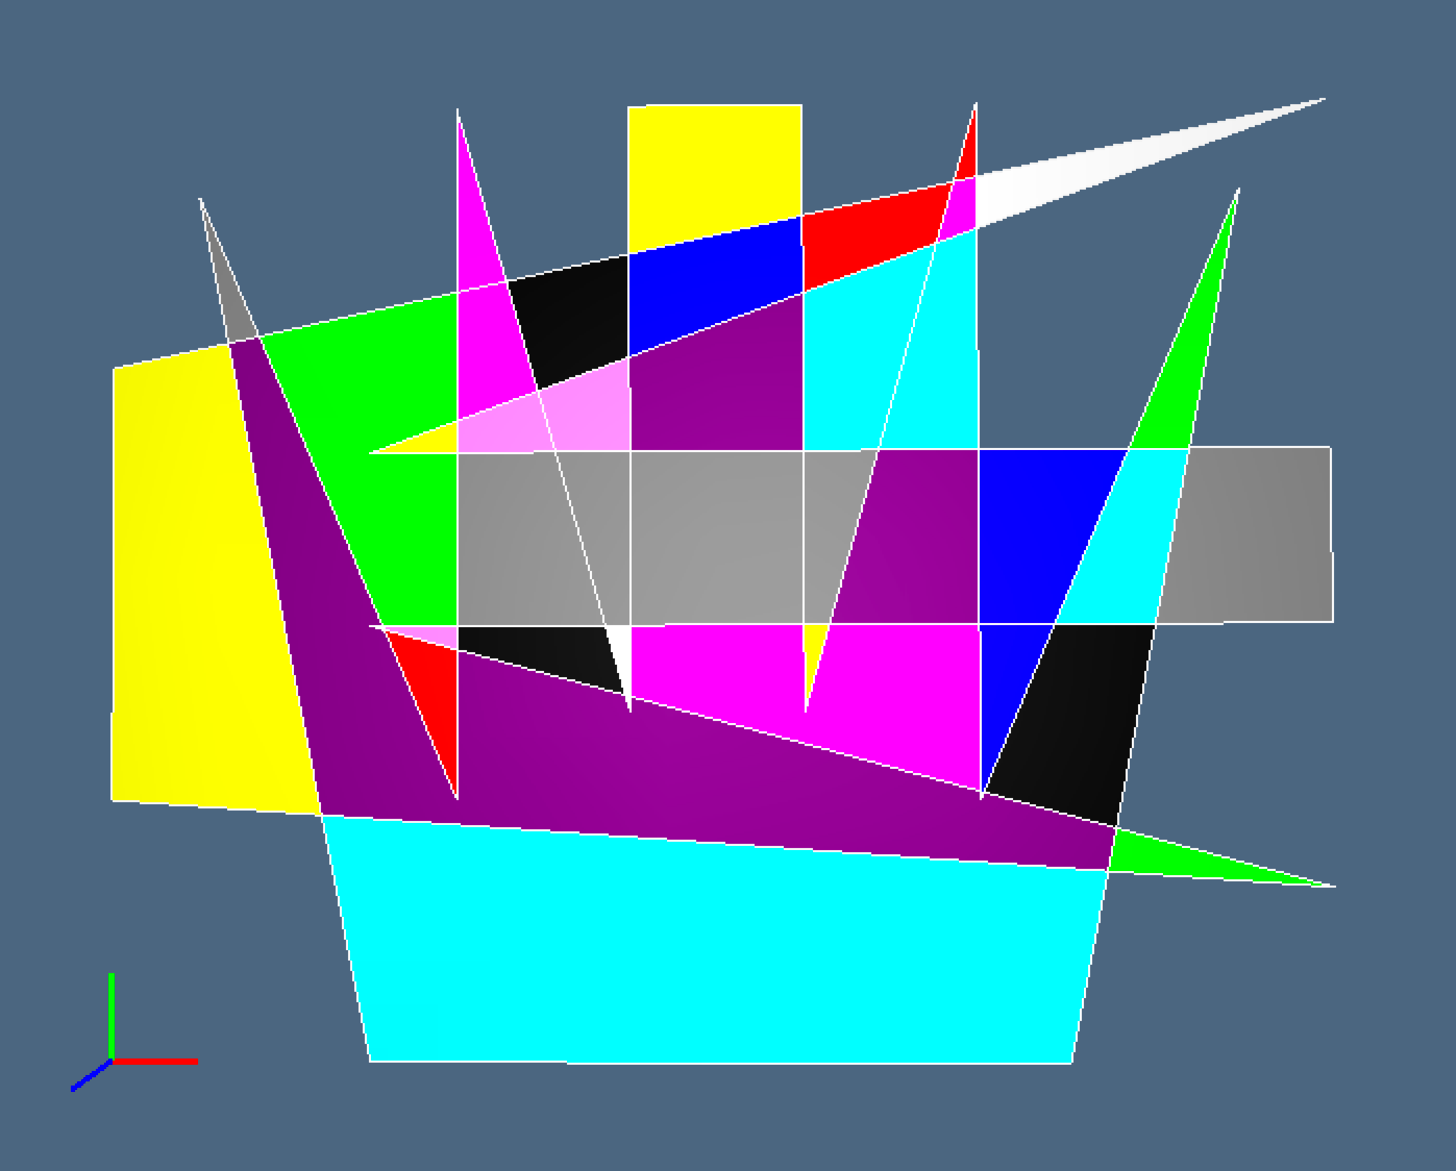
\includegraphics[height=0.2\linewidth,width=0.2425\linewidth]{images/fork3} 
   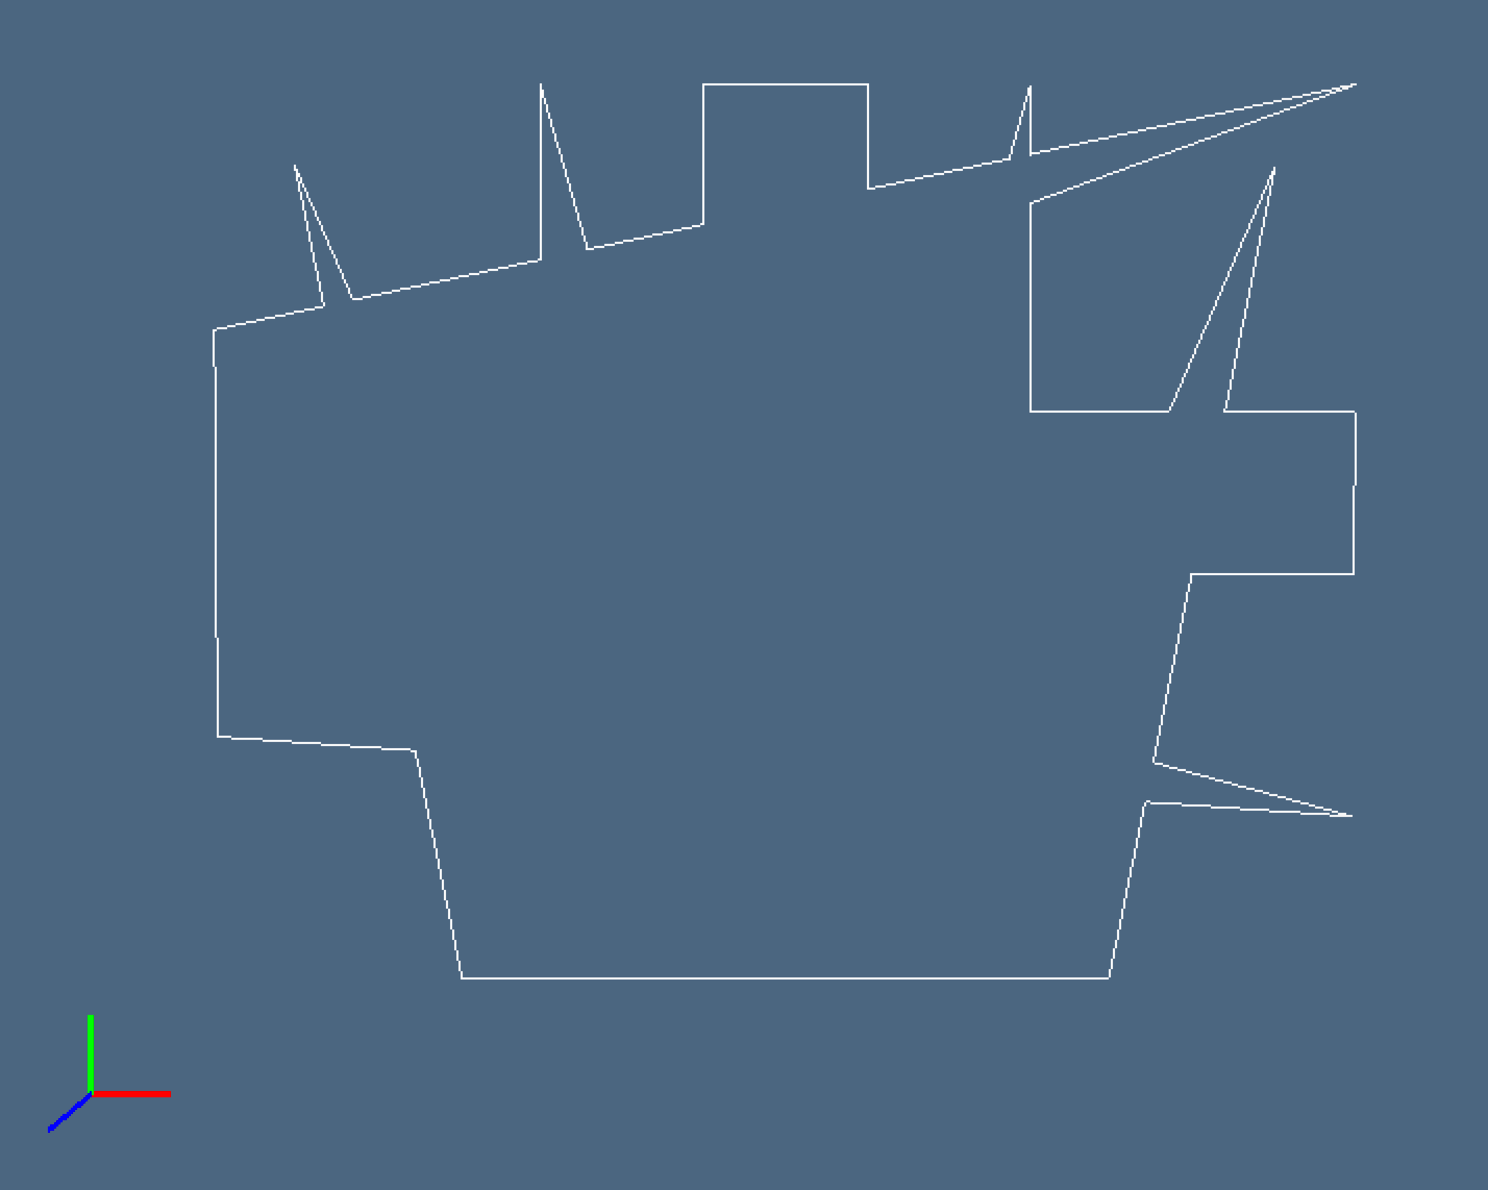
\includegraphics[height=0.2\linewidth,width=0.2425\linewidth]{images/fork4} 
   \caption{\texttt{LAR} complex from two polygons. (a) the input polygons; (b) the intersection of boundary lines; (c) the extracted \emph{regularized} 2-complex; (d) the boundary \texttt{LAR}.}
   \label{fig:ortho}
\end{figure}

%-------------------------------------------------------------------------------
@O test/py/bool2/test03.py
@{""" Boolean complex generated by boundaries of two complexes """
import sys
sys.path.insert(0, 'lib/py/')
from inters import *
glass = MATERIAL([1,0,0,0.1,  0,1,0,0.1,  0,0,1,0.1, 0,0,0,0.1, 100])

V1 = [[3,0],[11,0],[13,10],[10,11],[8,11],[6,11],[4,11],[1,10],[4,3],[6,4],
        [8,4],[10,3]]
FV1 = [[0,1,8,9,10,11],[1,2,11],[3,10,11],[4,5,9,10],[6,8,9],[0,7,8]]
EV1 = [[0,1],[0,7],[0,8],[1,2],[1,11],[2,11],[3,10],[3,11],[4,5],[4,10],[5,
        9],[6,8],[6,9],[7,8],[8,9],[9,10],[10,11]]
BE1 = boundaryCells(FV1,EV1)
lines1 = [[V1[v] for v in EV1[edge]] for edge in BE1]

V2 = [[0,3],[14,2],[14,5],[14,7],[14,11],[0,8],[3,7],[3,5]]
FV2 = [[0,5,6,7],[0,1,7],[4,5,6],[2,3,6,7]]
EV2 = [[0,1],[0,5],[0,7],[1,7],[2,3],[2,7],[3,6],[4,5],[4,6],[5,6],[6,7]]
BE2 = boundaryCells(FV2,EV2)
lines2 = [[V2[v] for v in EV2[edge]] for edge in BE2]

VIEW(STRUCT([ glass(STRUCT(MKPOLS((V1,FV1)))), glass(STRUCT(MKPOLS((V2,FV2)))) ]))
lines = lines1 + lines2
VIEW(STRUCT(AA(POLYLINE)(lines)))

global precision
PRECISION += 2
V,FV,EV = larFromLines(lines)
VIEW(EXPLODE(1.2,1.2,1)(MKPOLS((V,EV))))

VV = AA(LIST)(range(len(V)))
submodel = STRUCT(MKPOLS((V,EV)))
VIEW(larModelNumbering(1,1,1)(V,[VV,EV,FV[:-1]],submodel,1))

polylines = [[V[v] for v in face+[face[0]]] for face in FV[:-1]]
colors = [CYAN, MAGENTA, WHITE, RED, YELLOW, GREEN, GRAY, ORANGE, BLACK, BLUE, PURPLE, BROWN]
sets = [COLOR(colors[k%12])(FAN(pol)) for k,pol in enumerate(polylines)]
VIEW(STRUCT([ T(3)(0.02)(STRUCT(AA(POLYLINE)(lines))), STRUCT(sets)]))

VIEW(EXPLODE(1.2,1.2,1)((AA(POLYLINE)(polylines))))
polylines = [ [V[v] for v in FV[-1]+[FV[-1][0]]] ]
VIEW(EXPLODE(1.2,1.2,1)((AA(POLYLINE)(polylines))))
@}
%-------------------------------------------------------------------------------



\subsection{Testing the box-kd-trees}
%===============================================================================


\paragraph{Visualizing with different colors the buckets of box-kd-tree}
%-------------------------------------------------------------------------------
@O test/py/bool2/test04.py @{
""" Visualizing with different colors the buckets of box-kd-tree """
from pyplasm import *
""" import modules from larcc/lib """
import sys
sys.path.insert(0, 'lib/py/')
from bool2 import *

randomQuadArray = randomQuads(30,0.8)
VIEW(STRUCT(AA(MKPOL)([[verts, [[1,2,3,4]], None] for verts in randomQuadArray])))

boxes = containmentBoxes(randomQuadArray)
hexas = AA(box2exa)(boxes)
glass = MATERIAL([1,0,0,0.1,  0,1,0,0.1,  0,0,1,0.1, 0,0,0,0.1, 100])
yellow = STRUCT(AA(glass)(AA(MKPOL)([hex for hex,data in hexas])))
VIEW(STRUCT([#cyan,
    yellow]))

parts = boxBuckets(boxes)
for k,part in enumerate(parts):
    bunch = [glass(STRUCT( [MKPOL(hexas[h][0]) for h in part]))]
    bunch += [COLOR(RED)(MKPOL(hexas[k][0]))]
    VIEW(STRUCT(bunch))
@}
%-------------------------------------------------------------------------------


\subsection{Intersection of geometry subsets}
%===============================================================================


\paragraph{Two unit cubes}
%-------------------------------------------------------------------------------
@D Two unit cubes
@{""" Two unit cubes """
import sys
sys.path.insert(0, 'lib/py/')
from bool2 import *
glass = MATERIAL([1,0,0,0.1,  0,1,0,0.1,  0,0,1,0.1, 0,0,0,0.1, 100])

V,[VV,EV,FV,CV] = larCuboids([1,1,1],True)
cube1 = Struct([(V,FV,EV)],"cube1")
twoCubes = Struct([cube1,t(.5,.5,.5),cube1])
V,FV,EV = struct2lar(twoCubes)
VIEW(EXPLODE(1.2,1.2,1.2)(MKPOLS((V,FV))))

quadArray = [[V[v] for v in face] for face in FV]
boxes = containmentBoxes(quadArray)
hexas = AA(box2exa)(boxes)
parts = boxBuckets(boxes)
@}
%-------------------------------------------------------------------------------



\paragraph{Face (and incident faces) transformation}
%-------------------------------------------------------------------------------
@O test/py/bool2/test05.py
@{""" Face (and incident faces) transformation """

@< Two unit cubes @>

for k,bundledFaces in enumerate(parts):
    edges,faces = intersection(V,FV,EV)(k,bundledFaces)
    VIEW(STRUCT(edges + (AA)(COLOR(YELLOW))(faces)))
@}
%-------------------------------------------------------------------------------

k,face,FE[face] = 1 8 [14, 21, 20, 12] 
k,face,FE[face] = 1 10 [18, 22, 20, 16] 
k,face,FE[face] = 3 6 [13, 17, 16, 12] 
k,face,FE[face] = 3 10 [18, 22, 20, 16] 
k,face,FE[face] = 5 6 [13, 17, 16, 12] 
k,face,FE[face] = 5 8 [14, 21, 20, 12] 
k,face,FE[face] = 6 3 [3, 11, 10, 1] 
k,face,FE[face] = 6 5 [7, 11, 9, 5] 
k,face,FE[face] = 8 1 [3, 7, 6, 2] 
k,face,FE[face] = 8 5 [7, 11, 9, 5] 
k,face,FE[face] = 10 1 [3, 7, 6, 2] 
k,face,FE[face] = 10 3 [3, 11, 10, 1] 


\appendix
%===============================================================================
\section{Code utilities}
%===============================================================================

\paragraph{Coding utilities}

Some utility fuctions used by the module are collected in this appendix. Their macro names can be seen in the below script.

%-------------------------------------------------------------------------------
@D Coding utilities
@{""" Coding utilities """
@< Generation of a random 3D point @>
@< Generation of random 3D triangles @>
@< Generation of random 3D quadrilaterals @>
@< Generation of a single random triangle @>
@< Containment boxes @>
@< Transformation of a 3D box into an hexahedron @>
@< Computation of the 1D centroid of a list of 3D boxes @>
@}
%-------------------------------------------------------------------------------


\paragraph{Generation of random triangles}
The function \texttt{randomTriangles} returns the array \texttt{randomTriaArray} with a given number of triangles generated within the unit 3D interval. The \texttt{scaling} parameter is used to scale every such triangle, generated by three randow points, that could be possibly located to far from each other, even at the distance of the diagonal of the unit cube.

The arrays \texttt{xs}, \texttt{ys} and \texttt{zs}, that contain the $x,y,z$ coordinates of triangle points, are used to compute the minimal translation \texttt{v} needed to transport the entire set of data within the positive octant of the 3D space. 

%-------------------------------------------------------------------------------
@D Generation of random 3D triangles
@{""" Generation of random triangles """
def randomTriangles(numberOfTriangles=400,scaling=0.3):
    randomTriaArray = [rtriangle(scaling) for k in range(numberOfTriangles)]
    [xs,ys,zs] = TRANS(CAT(randomTriaArray))
    xmin, ymin, zmin = min(xs), min(ys), min(zs)
    v = array([-xmin,-ymin, -zmin])
    randomTriaArray = [[list(v1+v), list(v2+v), list(v3+v)] for v1,v2,v3 in randomTriaArray]
    return randomTriaArray
@}
%-------------------------------------------------------------------------------

\paragraph{Generation of random 3D quadrilaterals}

%-------------------------------------------------------------------------------
@D Generation of random 3D quadrilaterals
@{""" Generation of random 3D quadrilaterals """
def randomQuads(numberOfQuads=400,scaling=0.3):
    randomTriaArray = [rtriangle(scaling) for k in range(numberOfQuads)]
    [xs,ys,zs] = TRANS(CAT(randomTriaArray))
    xmin, ymin, zmin = min(xs), min(ys), min(zs)
    v = array([-xmin,-ymin, -zmin])
    randomQuadArray = [AA(list)([ v1+v, v2+v, v3+v, v+v2-v1+v3 ]) for v1,v2,v3 in randomTriaArray]
    return randomQuadArray
@}
%-------------------------------------------------------------------------------


\paragraph{Generation of a random 3D point}
A single random point, codified in floating point format, and with a fixed (quite small) number of digits, is returned by the \texttt{rpoint()} function, with no input parameters.
%-------------------------------------------------------------------------------
@D Generation of a random 3D point
@{""" Generation of a random 3D point """
def rpoint():
    return eval( vcode([ random.random(), random.random(), random.random() ]) )
@}
%-------------------------------------------------------------------------------
    
\paragraph{Generation of a single random triangle}
A single random triangle, scaled about its centroid by the \texttt{scaling} parameter, is returned by the \texttt{rtriangle()} function, as a tuple ot two random points in the unit square.
%-------------------------------------------------------------------------------
@D Generation of a single random triangle
@{""" Generation of a single random triangle """
def rtriangle(scaling):
    v1,v2,v3 = array(rpoint()), array(rpoint()), array(rpoint())
    c = (v1+v2+v3)/3
    pos = rpoint()
    v1 = (v1-c)*scaling + pos
    v2 = (v2-c)*scaling + pos
    v3 = (v3-c)*scaling + pos
    return tuple(eval(vcode(v1))), tuple(eval(vcode(v2))), tuple(eval(vcode(v3)))
@}
%-------------------------------------------------------------------------------
    

\paragraph{Containment boxes}

Given as input a list \texttt{randomTriaArray} of pairs of 2D points, the function \texttt{containmentBoxes} returns, in the same order, the list of \emph{containment boxes} of the input lines. A \emph{containment box} of a geometric object of dimension $d$ is defined as the minimal $d$-cuboid, equioriented with the reference frame, that contains the object. For a 2D line it is given by the tuple $(x1,y1,x2,y2)$, where $(x1,y1)$ is the point of minimal coordinates, and $(x2,y2)$ is the point of maximal  coordinates.

%-------------------------------------------------------------------------------
@D Containment boxes
@{""" Containment boxes """
def containmentBoxes(randomPointArray,qualifier=0):
    if len(randomPointArray[0])==2:
        boxes = [eval(vcode([min(x1,x2), min(y1,y2), min(z1,z2), 
                             max(x1,x2), max(y1,y2), max(z1,z2)]))+[qualifier]
                for ((x1,y1,z1),(x2,y2,z2)) in randomPointArray]
    elif len(randomPointArray[0])==3:
        boxes = [eval(vcode([min(x1,x2,x3), min(y1,y2,y3), min(z1,z2,z3), 
                             max(x1,x2,x3), max(y1,y2,y3), max(z1,z2,z3)]))+[qualifier]
                for ((x1,y1,z1),(x2,y2,z2),(x3,y3,z3)) in randomPointArray]
    elif len(randomPointArray[0])==4:
        boxes = [eval(vcode([min(x1,x2,x3,x4), min(y1,y2,y3,y4), min(z1,z2,z3,z4), 
                             max(x1,x2,x3,x4), max(y1,y2,y3,y4), max(z1,z2,z3,z4)]))+[qualifier]
                for ((x1,y1,z1),(x2,y2,z2),(x3,y3,z3),(x4,y4,z4)) in randomPointArray]
    return boxes
@}
%-------------------------------------------------------------------------------

    
\paragraph{Transformation of a 3D box into an hexahedron}
The transformation of a 2D box into a closed rectangular polyline, given as an ordered sequwncw of 2D points, is produced by the function \texttt{box2exa}
%-------------------------------------------------------------------------------
@D Transformation of a 3D box into an hexahedron
@{""" Transformation of a 3D box into an hexahedron """    
def box2exa(box):
    x1,y1,z1,x2,y2,z2,type = box
    verts = [[x1,y1,z1], [x1,y1,z2], [x1,y2,z1], [x1,y2,z2], [x2,y1,z1], [x2,y1,z2], [x2,y2,z1], [x2,y2,z2]]
    cell = [range(1,len(verts)+1)]
    return [verts,cell,None],type

def lar2boxes(model,qualifier=0):
    V,CV = model
    boxes = []
    for k,cell in enumerate(CV):
        verts = [V[v] for v in cell]
        x1,y1,z1 = [min(coord) for coord in TRANS(verts)]
        x2,y2,z2 = [max(coord) for coord in TRANS(verts)]
        boxes += [eval(vcode([min(x1,x2),min(y1,y2),min(z1,z2),max(x1,x2),max(y1,y2),max(z1,z2)]))+[(qualifier,k)]]
    return boxes
@}
%-------------------------------------------------------------------------------
    
\paragraph{Computation of the 1D centroid of a list of 3D boxes}
The 1D \texttt{centroid} of a list of 3D boxes is computed by the function given below.
The direction of computation (either $x,y$ or $z$) is chosen depending on the value of the \texttt{coord} parameter. 
%-------------------------------------------------------------------------------
@D Computation of the 1D centroid of a list of 3D boxes
@{""" Computation of the 1D centroid of a list of 3D boxes """    
def centroid(boxes,coord):
    delta,n = 0,len(boxes)
    ncoords = len(boxes[0])/2
    a = coord%ncoords
    b = a+ncoords
    for box in boxes:
        delta += (box[a] + box[b])/2
    return delta/n
@}
%-------------------------------------------------------------------------------

\bibliographystyle{amsalpha}
\bibliography{bool2}

\end{document}
